%Define a closed integral construct. I had some help with making this one look nice
\def\cint#1{\ensuremath{\displaystyle\underset{\substack{\text{\tiny{closed}}\\\text{\tiny{surface}}}}{\oint} \mspace{-0.1 mu} #1}}

%Define symbols for flux, just to make sure it stays consistent throughtout the paper
\def\phie{\ensuremath{\phi_E}}
\def\phib{\ensuremath{\phi_B}}

%Define the derivatives I'll be using, so I don't have to do all the typing every time
\def\dA{\ensuremath{\emph{d}\vec{A}}}
\def\dB{\ensuremath{\emph{d}\vec{B}}}
\def\ds{\ensuremath{\emph{d}\vec{s}}}
\def\dt{\ensuremath{\emph{dt}}}
\def\dphie{\ensuremath{\emph{d}\phie}}
\def\dphib{\ensuremath{\emph{d}\phib}}


\documentclass[a4paper]{article}
\title{Discretization and Numerical Solution of Partial Differential Equation}
\author{Luo Tao, Wenchao Zhang, Qikun Wu, Jiale Wang\\
South University of Science and Technology of China\\}
%\email{}
%\affiliation{South University of Science and Technology of China}

\usepackage{CJK,CJKnumb,CJKulem}
\usepackage{amsmath}
%\usepackage{amsthm}
\usepackage{amsfonts}
\usepackage{amssymb}
\usepackage[pdftex]{graphicx}
\usepackage{units}
\usepackage{graphicx}
\usepackage{esint}
\usepackage{subfigure}%插入并列的子图
\usepackage{multicol} %用于实现在同一页中实现不同的分栏
\usepackage{float}
\usepackage{geometry}%用于定义页边距
\usepackage{booktabs}
\usepackage{color}%修改字体颜色,示例用法见下
%\textcolor[rgb]{1.00,0,0}{cdscs}
%{\color{red}fcerfg}

\usepackage{times}%用于显示Latex风格的'\textsc{MatLab}'

\geometry{left=3cm,right=3cm,top=2.5cm,bottom=2.5cm}% 页边距定义


\newcommand\relphantom[1]{\mathrel{\phantom{#1}}}
\newcommand\ve{\varepsilon}  \newcommand\tve{t_{\varepsilon}}
\newcommand\vf{\varphi}      \newcommand\yvf{y_{\varphi}}
\newcommand\bfE{\mathbf{E}}


%以下用于让公式编号带有章节
%\makeatletter % `@' now normal "letter"
%\@addtoreset{equation}{section}
%\makeatother  % `@' is restored as "non-letter"
%\renewcommand\theequation{\oldstylenums{\thesection}.\oldstylenums{\arabic{equation}}}
%完毕-用于让公式编号带有章节

%以下用于让图片,表格,等号带有章节编号
\renewcommand\thefigure{\thesection.\arabic{figure}}
\renewcommand\thetable{\thesection.\arabic{table}}
\renewcommand\theequation{\thesection.\arabic{equation}}

%\addtolength{\textwidth}{1.2in}
%\addtolength{\textheight}{1.2in}
%\addtolength{\oddsidemargin}{-.58in}
%\addtolength{\evensidemargin}{-.58in}
%\renewcommand{\baselinestretch}{1.0}
\parindent = 0cm
%\parskip = .1cm

\newtheorem{theorem}{Theorem}
\newtheorem{acknowledgement}[theorem]{Acknowledgement}
\newtheorem{algorithm}[theorem]{Algorithm}
\newtheorem{axiom}[theorem]{Axiom}
\newtheorem{case}[theorem]{Case}
\newtheorem{claim}[theorem]{Claim}
\newtheorem{conclusion}[theorem]{Conclusion}
\newtheorem{condition}[theorem]{Condition}
\newtheorem{conjecture}[theorem]{Conjecture}
\newtheorem{corollary}[theorem]{Corollary}
\newtheorem{criterion}[theorem]{Criterion}
\newtheorem{definition}[theorem]{Definition}
\newtheorem{example}[theorem]{Example}
\newtheorem{exercise}[theorem]{Exercise}
\newtheorem{lemma}[theorem]{Lemma}
\newtheorem{notation}[theorem]{Notation}
\newtheorem{problem}[theorem]{Problem}
\newtheorem{proposition}[theorem]{Proposition}
\newtheorem{remark}[theorem]{Remark}
\newtheorem{solution}[theorem]{Solution}
\newtheorem{summary}[theorem]{Summary}
\newenvironment{proof}[1][Proof]{\textbf{#1.} }{\ \rule{0.5em}{0.5em}}



\usepackage{amsmath,amssymb,enumerate}

%%%%%%%%%% Start TeXmacs macros
\newcommand{\assign}{:=}
\newcommand{\tmem}[1]{{\em #1\/}}
\newcommand{\tmmathbf}[1]{\ensuremath{\boldsymbol{#1}}}
\newcommand{\tmname}[1]{\textsc{#1}}
\newcommand{\tmop}[1]{\ensuremath{\operatorname{#1}}}
\newcommand{\tmstrong}[1]{\textbf{#1}}
\newcommand{\tmtextbf}[1]{{\bfseries{#1}}}
\newcommand{\tmtextit}[1]{{\itshape{#1}}}
\newcommand{\tmtextup}[1]{{\upshape{#1}}}
\newenvironment{enumeratenumeric}{\begin{enumerate}[1.] }{\end{enumerate}}
\newenvironment{enumerateromancap}{\begin{enumerate}[I.] }{\end{enumerate}}
\newenvironment{itemizedot}{\begin{itemize} \renewcommand{\labelitemi}{$\bullet$}\renewcommand{\labelitemii}{$\bullet$}\renewcommand{\labelitemiii}{$\bullet$}\renewcommand{\labelitemiv}{$\bullet$}}{\end{itemize}}
\newenvironment{tmindent}{\begin{tmparmod}{1.5em}{0pt}{0pt} }{\end{tmparmod}}
\newenvironment{tmparmod}[3]{\begin{list}{}{\setlength{\topsep}{0pt}\setlength{\leftmargin}{#1}\setlength{\rightmargin}{#2}\setlength{\parindent}{#3}\setlength{\listparindent}{\parindent}\setlength{\itemindent}{\parindent}\setlength{\parsep}{\parskip}} \item[]}{\end{list}}
\newenvironment{tmparsep}[1]{\begingroup\setlength{\parskip}{#1}}{\endgroup}

\AtBeginDocument
{\begin{CJK*}{GBK}{song} % 不计中文的空格
\CJKindent                           % 首行缩进两个汉字
\sloppy\CJKspace                     % 中英文混排的断行
%\CJKtilde                            % 重新定义~用~隔开中英文
%\CJKcaption{GB}                      % 章节标题的中文化
}
\AtEndDocument{\end{CJK*}}

\begin{document}

\maketitle
\tableofcontents
\newpage

\begin{abstract}
A thorough exploration of discretization method and \textsc{MatLab} implementation of PDE is illustrated. Methods of Dirichlet, Neumann, Forward-Difference and Crank-Nicolson are presented in detail to deal with three kinds of PDE: Hyperbolic, Parabolic and Elliptic. Besides, a general solution Runge-Kutta method is showed to solve ODE system after the discretization of PDE.
\end{abstract}

\section{Background of PDE}

\subsection{Hyperbolic Equation}
Equation 
\begin{equation}
\frac{d^{2}u}{dt^{2}}=c^{2}\nabla^{2}u
\end{equation}
 is called a hyperbolic equation.

\subsubsection{wave propagation}
consider the longitudinal wave propagating in a rod, we divide it into infinitesimal elements. for each element $i|i=1.2...n$ start from $x_{i}$to $x_{i+1}$, equation of motion is
\begin{equation}
\unit{m_{i}\frac{d^{2}u}{dt^{2}}=k(u_{i+1}-u_{i})-(u_{i}-u_{i-1})}
\end{equation}
where $u$ is the displacement along the rod.as $K=k/N,\triangle x=l/N,m_{i}=M/N$,
we get 
\[\frac{d^{2}u}{dt^{2}}=\frac{KL^{2}}{M}\frac{(u_{i+1}-2u_{i}+u_{i-1})}{\triangle x^{2}}\]
which becomes 
\begin{equation}
\frac{d^{2}u}{dt^{2}}=\frac{KL^{2}}{M}\frac{d^{2}u}{dx^{2}}
\end{equation}
when $n\rightarrow+\infty$

\begin{figure}[!htb]
\centering
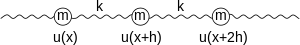
\includegraphics[width=10cm]{longitude_wave.png}
%\caption{ploy of $Q(x)$}
%\label{eval_2}
\end{figure}

\subsubsection{Transverse Wave Propagation}
In Fig~\ref{TWP}, consider the transverse wave propagating in a string,assume the
tension is $f$, and vibration don't have a spatial frequency such
that $u_{x}$is small enough. we divide it into infinitesimal elements.
for each point $i$, the net force perpendicular to string is $\frac{f}{\Delta x}(u_{i-1}-2u_{i}+u_{i+1})$,
pay attention that here we use the approximation $\cos\left(\theta\right)\approx tan(\theta)$
as $\theta\rightarrow0$.equation of motion holds
\[m_{i}\frac{d^{2}u}{dt^{2}}=\frac{f}{\Delta x}(u_{i-1}-2u_{i}+u_{i+1})\]
replace $m_{i}$ by $\Delta x\rho$ and let $\Delta x\rightarrow0$, we get 
\begin{equation}
\frac{d^{2}u}{dt^{2}}=\frac{f}{\rho}\frac{d^{2}u}{dx^{2}}
\end{equation}



\begin{figure}[!htb]
\centering
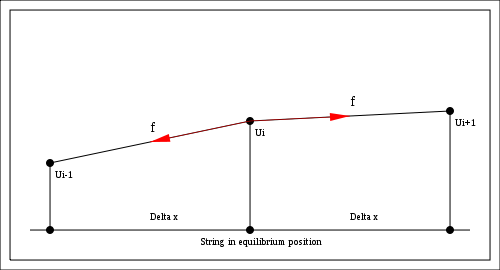
\includegraphics[width=10cm]{500px-String_wave_0.png}
\caption{String Motion in Equilibrium}
\label{TWP}
\end{figure}
\subsubsection{High dimension Wave  Propagation}
Similarly, in high dimension case, wave function become $\frac{d^{2}u}{dt^{2}}=c^{2}\nabla^{2}u$
where $c^{2}$is a positive constant.

\subsection{Parabolic Equation}

Equation 
\begin{equation}
\frac{du}{dt}=\alpha\nabla^{2}u
\end{equation} 
where $\alpha$ is a positive constant, is called a parabolic equation (also heat equation).
\\\\
By Fourier's Law$V_{q}=-k\nabla u$, take the surface integral on
both sides we get 
\begin{equation}
\oiint V_{q}d\sigma=-k\oiint\nabla ud\sigma
\label{1.1}
\end{equation}
The left side means the heat flow out of the surface i.e. $-\iiint q_{t}dv$.
\\The right side, by Gauss's Law, can be written as volumn integral
$-k\iiint\nabla^{2}udv$. On the other side, $\Delta q=c_{p}\rho\Delta u$
hence $q_{t}=c_{p}\rho u_{t}$.so just by arranging equation~\ref{1.1},it becomes
\begin{equation}
u_{t}=\frac{k}{c_{p}\rho}\nabla^{2}u
\end{equation} 
where $\frac{k}{c_{p}\rho}=\alpha$.

heat function can also appear in difusion problem, the only difference
is to consider $u$ to be particle number density.the famous Schrodinger
equation for a free particle is also heat equation basicly, except
that $\alpha$ here is a complex number.

\subsection{Elliptic Equation}


Laplace equation 
\begin{equation}
\Delta\varphi=0
\end{equation}
and Possion equation
\begin{equation}
\Delta\varphi=f
\end{equation}
are both elliptic equation.
\\\\
In Electrostatics, $\varphi$is electrical potential and $\Delta\varphi$means
charge density. So above equation means no charge case and charge
with $f$ distribution case.
\\
In Newtonian gravity, $f$ is density and $\varphi$is gravitational
potential.

\section{Definite Problem of Partial Differential Equation}

\subsection{Elliptical Partial Differential Equation}

\ \ \ The process that fixes time can be described as an elliptical partial
differential equation.The most typical and simplest form of elliptical
equation is Poisson's equation
\begin{equation}
  \Delta u = \frac{\partial^2 u}{\partial x^2} + \frac{\partial^2 u}{\partial
  y^2} = f \left( x, y \right)
\end{equation}
\ \ \ \ Particularly,if $f \left( x, y \right) \equiv 0$,then the equation is
called Laplace's equation.

More over, if we give some definite conditions to the equation then the
problem become definite problem.Such definite conditions are initial condition
and boundary condition.The boundary value problem of Poisson equation is
{\cite{Lu&Guan}}
\[ \left\{ \begin{array}{lr}
     \frac{\partial^2 u}{\partial x^2} + \frac{\partial^2 u}{\partial y^2} = f
     \left( x, y \right)  & \left( x, y \right) \in \Omega\\
     u \left( x, y \right) \left|_{\left( x, y \right) \in \Gamma} = \right.
     \varphi \left( x, y \right) & \Gamma = \partial \Omega
   \end{array} \right. \]
\ \ \ \ where $\Omega$ is a bounded(by $\Gamma$) area, $\Gamma$ is segmental
smooth curve.$f \left( x, y \right)$ and $\varphi \left( x, y \right)$ are
continous function.

Another famous elliptical partial differential equation is Helmholtz
equation:$\Delta u + f \left( x, y \right) u = g \left( x, y
\right)${\cite{Peaceman&Rachford}}
.

\subsection{Parabolic Partial Differential Equation}

\ \ \ \ When we study the problem like heat conduction,we may face such
parabolic equation.The simplest form of parabolic equation is one order form
parabolic equation:
\begin{equation}
  \frac{\partial u}{\partial t} - a \frac{\partial^2 u}{\partial x^2} = 0
  \left( a > 0 \right) \label{para}
\end{equation}
\ \ \ Equation \ref{para} has two different definite problem: initial value
problem(Cauchy Problem) and initial boudary value problem:
\begin{enumeratenumeric}
  \item Initial Value Problem(IVP)
  \begin{equation}
    \left\{ \begin{array}{ll}
      \frac{\partial u}{\partial t} - a \frac{\partial^2 u}{\partial x^2} = 0
      & t > 0, - \infty < x < + \infty\\
      u \left( x, 0 \right) = \varphi \left( x \right) & - \infty < x < +
      \infty
    \end{array} \right.
  \end{equation}
  \item Initial Boundary Value Problem(BVP)
  \begin{equation}
    \left\{ \begin{array}{ll}
      \frac{\partial u}{\partial t} - a \frac{\partial^2 u}{\partial x^2} = 0
      & 0 < t < T, 0 < x < l\\
      u \left( x, 0 \right) = \varphi \left( x \right) & 0 \leqslant x
      \leqslant l\\
      u \left( 0, t \right) = g_1 \left( t \right), u \left( l, t \right) =
      g_2 \left( t \right) & 0 \leqslant t \leqslant T
    \end{array} \right.
  \end{equation}
\end{enumeratenumeric}
\ \ \ \ \ \ \ where $\varphi \left( x \right), g_1 \left( x \right), g_2
\left( x \right)$ are known and $\varphi \left( 0 \right) = g_1 \left( 0
\right), \varphi \left( l \right) = g_2 \left( 0 \right)$.

\subsection{Hyperbolic Partial Differential Equation}

\ \ \ \ Wave equation is a classic form of Hyperbolic equation with two
order.The simplest form of hyperbolic equation is one order form:
\begin{equation}
  \frac{\partial u}{\partial t} + a \frac{\partial^{} u}{\partial x} = 0
\end{equation}
\ \ \ \ The form we are familiar in physical: one dimensional shock and wave
equation is following:
\begin{equation}
  \frac{\partial^2 u}{\partial t^2} = a^2 \frac{\partial^2 u}{\partial x^2}
\end{equation}
\ \ \ \ Similarly with Parobolic form,we have IVP and BVP:
\begin{enumeratenumeric}
  \item Initial Value Problem(IVP)
  \begin{equation}
    \left\{ \begin{array}{ll}
      \frac{\partial^2 u}{\partial t^2} = a^2 \frac{\partial^2 u}{\partial
      x^2} & t > 0, - \infty < x < + \infty\\
      u \left( x, 0 \right) = \varphi \left( x \right) & - \infty < x < +
      \infty\\
      \frac{\partial u}{\partial t} |_{t = 0} = \phi \left( x \right) & -
      \infty < x < + \infty
    \end{array} \right.
  \end{equation}
  \item Initial Boundary Value Problem(BVP)
  \begin{equation}
    \left\{ \begin{array}{ll}
      \frac{\partial^2 u}{\partial t^2} = a^2 \frac{\partial^2 u}{\partial
      x^2} & t > 0, 0 < x < l\\
      u \left( x, 0 \right) = \varphi \left( x \right), \frac{\partial
      u}{\partial t} |_{t = 0} = \phi \left( x \right) & 0 \leqslant x
      \leqslant l\\
      u \left( 0, t \right) = g_1 \left( t \right), u \left( l, t \right) =
      g_2 \left( t \right) & 0 \leqslant t \leqslant T
    \end{array} \right.
  \end{equation}
\end{enumeratenumeric}
\ \ \ \ \ \ \ where $\varphi \left( x \right), g_1 \left( x \right), g_2
\left( x \right)$ are known and $\varphi \left( 0 \right) = g_1 \left( 0
\right), \varphi \left( l \right) = g_2 \left( 0 \right)$.


\section{solution to ODE system {\cite{Teschl}}{\cite{He&Peng}}}

\subsection{matrix multiplication}
\subsubsection{norm}

Let $X$ be a real vector space. A norm on $X$ is a map $\left\| . \right\|:X\to [0,\infty )$ satisfying the following requirements:

\begin{enumerateromancap}
  \item $\left\| 0 \right\|=0,\left\| x \right\|>0$ for$x\in X\backslash \{0\}$
  \item $\left\| \lambda x \right\|=\left| \lambda  \right|\left\| x \right\|$ for $\lambda \in \mathbb{R}$ and $x\in X$
  \item $\left\| x+y \right\|\le \left\| x \right\|+\left\| y \right\|$for$x,y\in X$
\end{enumerateromancap}

The pair $\left( X,\left\| . \right\| \right)$  is called a normed vector space. Given a normed vector space $X$, we have the concept of convergence and of a Cauchy sequence in this space. The normed vector space is called complete if every Cauchy sequence converges. A complete normed vector space is called a Banach space.
For any vector $x$, three kinds of norm (1-norm, 2-norm and $\infty$-norm) are usually used. In general, the p-norm of a vector is represented as:

\begin{equation}
{{\left\| x \right\|}_{p}}={{\left[ \sum\limits_{i=1}^{n}{{{\left| {{x}_{i}} \right|}^{p}}} \right]}^{\frac{1}{p}}}
\end{equation}
Since ${{\mathbb{C}}^{n}}$ is algebraically closed, we use ${{\mathbb{C}}^{n}}$  as underlying vector space rather than ${{\mathbb{R}}^{n}}$.

The norm of matrix is introduced as follows:
\begin{equation}
\left\| \mathbf{A} \right\|=\underset{x:\left| x \right|=1}{\mathop{\sup }}\,\left| \mathbf{A}x \right|
\end{equation}
We can then see that the space of $n\times n$ matrices becomes a Banach space.
Since matrix norm is just a kind of norm, we can see that it also satisfy the nature of norm:

\begin{enumerateromancap}
  \item $\left\| \mathbf{0} \right\|=0,\left\| \mathbf{A} \right\|>0$ for$\mathbf{A}\in \mathbf{L}({{\mathbf{R}}^{n}})\backslash \{\mathbf{0}\}$
  \item $\left\| \lambda \mathbf{A} \right\|=\left| \lambda  \right|\left\| \mathbf{A} \right\|$ for $\lambda \in \mathbf{R}$ and $\mathbf{A}\in \mathbf{L}({{\mathbf{R}}^{n}})$
  \item $\left\| \mathbf{A+B} \right\|\le \left\| \mathbf{A} \right\|+\left\| \mathbf{B} \right\|$for$\mathbf{A},\mathbf{B}\in \mathbf{L}({{\mathbf{R}}^{n}})$
\end{enumerateromancap}

So we have following Lemma:
\begin{lemma}
for $\forall \mathbf{A},\mathbf{B}\in \mathbf{L}({{\mathbf{R}}^{n}})$ and $x\in {{\mathbf{R}}^{n}}$:
\begin{enumerateromancap}
  \item $\left| \mathbf{A}x \right|\le \left\| \mathbf{A} \right\|\left| x \right|$
  \item $\left\| \mathbf{AB} \right\|\le \left\| \mathbf{A} \right\|\left\| \mathbf{B} \right\|$
  \item $\left\| {{\mathbf{A}}^{k}} \right\|\le {{\left\| \mathbf{A} \right\|}^{k}}$
\end{enumerateromancap}
\end{lemma}
\ \\
\begin{proof}\\
(i)by definition,
$\left\| \mathbf{A} \right\|\ge \left| \mathbf{A}\frac{x}{\left| x \right|} \right|=\frac{\left| \mathbf{A}x \right|}{\left| x \right|}$\\
(ii)from (i) we have for $\left| x \right|\le 1$ :
\[\left| \mathbf{AB}x \right|\le \left\| \mathbf{A} \right\|\left| \mathbf{B}x \right|\le \left\| \mathbf{A} \right\|\left\| \mathbf{B} \right\|\left| x \right|\]\\
(iii) from (ii)we can easily proof use deduction
\end{proof}

So the convergence of the series $\sum\limits_{k=0}^{\infty }{\frac{{{\mathbf{A}}^{k}}}{k!}}$ can be proofed in the following theorem:
\begin{theorem}
\label{convergence_of_exp(A)}
For $\forall \mathbf{A}\in \mathbf{L}({{\mathbf{R}}^{n}})$ and ${{t}_{0}}>0$ , \[\sum\limits_{k=0}^{\infty }{\frac{{{\mathbf{A}}^{k}}{{t}^{k}}}{k!}}\]converge uniformly for $\forall \left| t \right|<{{t}_{0}}$
\end{theorem}
The theorem is easily proofed by using \[\left\| {{\mathbf{A}}^{k}} \right\|\le {{\left\| \mathbf{A} \right\|}^{k}}\]
We can then define matrix exponential.

\subsubsection{matrix exponential}
A matrix exponential of a matrix $A$ is given by:
\[{{e}^{\mathbf{A}}}=\exp (\mathbf{A})=\sum\limits_{i=0}^{\infty }{\frac{1}{i!}{{\mathbf{A}}^{i}}}\]
However, note that in general,
$\exp (\mathbf{A}+\mathbf{B})\ne \exp (\mathbf{A})\exp (\mathbf{B})$
Unless the communicator $[\mathbf{A,B}]=\mathbf{AB-BA}=\mathbf{0}$
By the theorem ~\ref{convergence_of_exp(A)}, we can see that $\exp (\mathbf{A})=\sum\limits_{i=0}^{\infty }{\frac{1}{i!}{{\mathbf{A}}^{i}}}$converge for $\forall \mathbf{A}$ . Moreover, we can have some properties:
\\\\
(i) if $\mathbf{B=PA}{{\mathbf{P}}^{\mathbf{-1}}}$ then ${{e}^{\mathbf{B}}}\mathbf{=P}{{e}^{\mathbf{A}}}{{\mathbf{P}}^{\mathbf{-1}}}$\\\\
(ii) if $\mathbf{A}=\mathbf{P}diag\left( {{\lambda }_{j}} \right){{\mathbf{P}}^{\mathbf{-1}}}$, then ${{e}^{\mathbf{A}t}}=\mathbf{P}diag\left( {{e}^{{{\lambda }_{j}}t}} \right){{\mathbf{P}}^{-1}}$\\\\
The first property can be done easily by calculation:
\[{{e}^{\mathbf{B}}}\mathbf{=}\exp (\mathbf{B})=\sum\limits_{i=0}^{\infty }{\frac{1}{i!}{{\mathbf{B}}^{i}}}=\sum\limits_{i=0}^{\infty }{\frac{1}{i!}{{\left( \mathbf{PA}{{\mathbf{P}}^{\mathbf{-1}}} \right)}^{i}}}=\sum\limits_{i=0}^{\infty }{\frac{1}{i!}\mathbf{P}{{\mathbf{A}}^{i}}{{\mathbf{P}}^{\mathbf{-1}}}}=\mathbf{P}{{e}^{\mathbf{A}}}{{\mathbf{P}}^{\mathbf{-1}}}\]
And the second property can be directly gained from the first property.

\subsubsection{Jordan canonical form{\cite{Zhang&Xu}}}
We can use Jordan canonical form to solve a wide range of ODE system $x’=Ax$
\begin{theorem}
(Cayley-Hamilton) Every matrix satisfies its own characteristic equation
\begin{equation}
{{\chi }_{A}}(\mathbf{A})=0
\end{equation}
\end{theorem}
\ \\
\begin{proof}
Assume that ${{\alpha }_{1}},{{\alpha }_{2}},\ldots {{\alpha }_{n}}$ is the base of linear space $V$, and $A$ is the matrix representation of linear transformation $\textbf{A}$, then we have:
\begin{equation}
(\textbf{A}{{\alpha }_{1}},\textbf{A}{{\alpha }_{2}},\ldots \textbf{A}{{\alpha }_{n}})=({{\alpha }_{1}},{{\alpha }_{2}},\ldots {{\alpha }_{n}})A
\end{equation}
Which can be written as:
\begin{equation}
\left( \begin{matrix}
   \textbf{A} & {} & {} & {}  \\
   {} & \textbf{A} & {} & {}  \\
   {} & {} & \ddots  & {}  \\
   {} & {} & {} & \textbf{A}  \\
\end{matrix} \right)\left( \begin{matrix}
   {{\alpha }_{1}}  \\
   {{\alpha }_{2}}  \\
   \vdots   \\
   {{\alpha }_{n}}  \\
\end{matrix} \right)={{A}^{T}}\left( \begin{matrix}
   {{\alpha }_{1}}  \\
   {{\alpha }_{2}}  \\
   \vdots   \\
   {{\alpha }_{n}}  \\
\end{matrix} \right)
\end{equation}
We denote the equation above as:
\begin{equation}
\left( \begin{matrix}
   \lambda  & {} & {} & {}  \\
   {} & \lambda  & {} & {}  \\
   {} & {} & \ddots  & {}  \\
   {} & {} & {} & \lambda   \\
\end{matrix} \right)\left( \begin{matrix}
   {{\alpha }_{1}}  \\
   {{\alpha }_{2}}  \\
   \vdots   \\
   {{\alpha }_{n}}  \\
\end{matrix} \right)={{A}^{T}}\left( \begin{matrix}
   {{\alpha }_{1}}  \\
   {{\alpha }_{2}}  \\
   \vdots   \\
   {{\alpha }_{n}}  \\
\end{matrix} \right)
\end{equation}
Then we simply have:
\begin{equation}
(\lambda I-{{A}^{T}})\left( \begin{matrix}
   {{\alpha }_{1}}  \\
   {{\alpha }_{2}}  \\
   \vdots   \\
   {{\alpha }_{n}}  \\
\end{matrix} \right)=0,{{\chi }_{A}}(A)=\det \left| \lambda I-{{A}^{T}} \right|=0
\end{equation}
\end{proof}
\\
The aim of Jordan canonical form is to decompose the linear space. We first should spilt our space into some subspace and then apply a more accurate decomposition to each subspace.
\begin{definition}
(generalized eigenspace)\\ A generalized eigenspace is the kernel of polynomial $f(\lambda )$ :\\
$\ker f=\ker f(\lambda )=\{\alpha \in V|f(\textbf{A})\alpha =0\}$
\end{definition}

Under such definition, we can first apply a primary decomposition to our linear space $V$:
\begin{theorem}
(primary decomposition) \\
let $m(\lambda )$ be the minimal annihilator of linear space $V$ on field $F$.
\begin{equation}
m(\lambda )={{p}_{1}}{{(\lambda )}^{{{r}_{1}}}}{{p}_{2}}{{(\lambda )}^{{{r}_{2}}}}\ldots {{p}_{s}}{{(\lambda )}^{{{r}_{s}}}}
\end{equation}
Then the generalized eigenspace of ${{p}_{i}}{{(\lambda )}^{{{r}_{i}}}}$, saying $W_i$, is an invariant subspace of $V$ and
\begin{equation}
V={{W}_{1}}\oplus {{W}_{2}}\oplus \ldots \oplus {{W}_{s}}
\end{equation}
\end{theorem}

The proof is omitted since it is not what we are focus on.
After the primary decomposition, we know that the characteristic equation of a $n\times n$ matrix $A$ can be written as

\begin{equation}
f(\lambda )={{(\lambda -{{\lambda }_{1}})}^{{{d}_{1}}}}{{(\lambda -{{\lambda }_{2}})}^{{{d}_{2}}}}\ldots {{(\lambda -{{\lambda }_{s}})}^{{{d}_{s}}}}
\end{equation}
where ${{d}_{1}}+{{d}_{2}}+\ldots +{{d}_{s}}=n$. Moreover, the minimal annihilator is
\begin{equation}
m(\lambda )={{(\lambda -{{\lambda }_{1}})}^{{{r}_{1}}}}{{(\lambda -{{\lambda }_{2}})}^{{{r}_{2}}}}\ldots {{(\lambda -{{\lambda }_{s}})}^{{{r}_{s}}}}
\end{equation}
where ${{r}_{i}}\le {{d}_{i}}$ for $i=1\ldots s$
Our target is to find the Jordan canonical form $J$ and the $P$ satisfying ${{P}^{-1}}AP=J$. The method can be illustrated in the following way:


\begin{enumerateromancap}
  \item Write down the characteristic equation $f(\lambda )$ of $A$. we have
  \[f(\lambda )={{(\lambda -{{\lambda }_{1}})}^{{{d}_{1}}}}{{(\lambda -{{\lambda }_{2}})}^{{{d}_{2}}}}\ldots {{(\lambda -{{\lambda }_{s}})}^{{{d}_{s}}}},\sum{{{d}_{i}}}=n\]
   Then we can know that
   \[A\sim diag\{{{J}_{{{d}_{1}}}}({{\lambda }_{1}}),{{J}_{{{d}_{2}}}}({{\lambda }_{2}}),\ldots ,{{J}_{{{d}_{s}}}}({{\lambda }_{s}})\}=J\]
  \item Then we look into ${{J}_{{{d}_{i}}}}({{\lambda }_{i}})$. We know that ${{J}_{{{d}_{i}}}}({{\lambda }_{i}})$ is consists of several Jordan blocks. Furthermore, the number of Jordan blocks is the number of linear independent eigenvector whose eigenvalue is ${{\lambda }_{i}}$. This number also equals to the dimension of $\ker (A-\lambda I)$ .
  \item After we know the number of Jordan blocks for each eigenvalue, we should exactly know the number of $k\times k$ Jordan block ${{N}_{k,{{\lambda }_{i}}}}$  which eigenvalue is ${{\lambda }_{i}}$. We have:
      \[{{N}_{k,{{\lambda }_{i}}}}=[rank{{(A-{{\lambda }_{i}}I)}^{k-1}}-rank{{(A-{{\lambda }_{i}}I)}^{k}}]-[rank{{(A-{{\lambda }_{i}}I)}^{k}}-rank{{(A-{{\lambda }_{i}}I)}^{k+1}}]\]
    \item We choose a set of vector $\left\{ a \right\}$ which satisfies
    \[a\in \ker {{(A-\lambda I)}^{k}},a\notin \ker {{(A-\lambda I)}^{k-1}}\]
And gain a Jordan chain
\[{{a}_{j}},(A-{{\lambda }_{i}}I){{a}_{j}},\ldots ,{{(A-{{\lambda }_{i}}I)}^{k-1}}{{a}_{j}}\]
 for each ${{a}_{j}}\in \left\{ a \right\}$. Then for all eigenvalues, the Jordan chain produce the $P$ we wanted.
\end{enumerateromancap}




\subsection{Solution to ODE systems}
\subsubsection{homogeneous linear system $x'=Ax$}
We first consider the scenario that our first order linear ODEs system is in the form $\mathbf{x'=Ax}$ where $\mathbf{A}$ is time-independent. Like the first order ODE and second order ODE, there is theorem claims about the existence and uniqueness of the solution:
\begin{theorem}
(Existence and uniqueness) $\mathbf{A}$ is a $n\times n$ matrix which is time-independent. Then for $\forall {{\mathbf{x}}_{\mathbf{0}}}\in {{\mathbf{R}}^{n}}$, there exist a unique solution to initial value problem for

\begin{eqnarray}     %方程组开始
\left\{                        %方程组的左边包括大括号\{
\begin{array}{lll}       %设定列阵的格式:{lll}是三个L,表示三列的对齐方式为Left对齐
\mathbf{x}'\mathbf{=Ax} \\
\mathbf{x}(0)={{\mathbf{x}}_{\mathbf{0}}} \\
\end{array}              %方程列阵的结束
\right.                       %方程组的右边无符号,利用“.“来标示
\end{eqnarray}

And the solution is:
$\mathbf{x}(t)={{e}^{\mathbf{A}t}}{{\mathbf{x}}_{\mathbf{0}}}$
\end{theorem}
The proof of the theorem require the flowing lemma:

\begin{lemma}
$\frac{d}{dt}{{e}^{\mathbf{A}t}}=\mathbf{A}{{e}^{\mathbf{A}t}}$
\end{lemma}
\begin{proof}\\
$\frac{d}{dt}{{e}^{\mathbf{A}t}}=\underset{\Delta t\to 0}{\mathop{\lim }}\,\frac{{{e}^{\mathbf{A}(t+\Delta t)}}-{{e}^{\mathbf{A}t}}}{\Delta t}={{e}^{\mathbf{A}t}}\underset{\Delta t\to 0}{\mathop{\lim }}\,\frac{{{e}^{\mathbf{A}\Delta t}}-I}{\Delta t}={{e}^{\mathbf{A}t}}\underset{\Delta t\to 0}{\mathop{\lim }}\,\sum\limits_{i=1}^{\infty }{\frac{1}{i!}{{\mathbf{A}}^{i}}\Delta {{t}^{i-1}}}={{e}^{\mathbf{A}t}}\mathbf{A}$
\end{proof}
\\\\
Now use this lemma we can proof the theorem we mentioned above:\\\\
\begin{proof}
\\(Existence) Using the lemma, if $\mathbf{x}(t)={{e}^{\mathbf{A}t}}{{\mathbf{x}}_{\mathbf{0}}}$ then
$\frac{d}{dt}\mathbf{x}(t)=\frac{d}{dt}{{e}^{\mathbf{A}t}}{{\mathbf{x}}_{\mathbf{0}}}=\mathbf{A}{{e}^{\mathbf{A}t}}{{\mathbf{x}}_{\mathbf{0}}}=\mathbf{Ax}(t)\ for\ \forall t\in \mathbf{R}$
And $\mathbf{x}(0)=I{{\mathbf{x}}_{\mathbf{0}}}={{\mathbf{x}}_{\mathbf{0}}}$. So $\mathbf{x}(t)={{e}^{\mathbf{A}t}}{{\mathbf{x}}_{\mathbf{0}}}$ is indeed a solution to the IVP. The existence is then been proofed.
\\(Uniqueness) we assume that there exist another solution to such IVP, let’s say it is $\mathbf{z}(t)$. We let $\mathbf{y}(t)={{e}^{-\mathbf{A}t}}\mathbf{z}(t)$, then:
$\mathbf{y}'(t)=-\mathbf{A}{{e}^{-\mathbf{A}t}}\mathbf{z}(t)+{{e}^{-\mathbf{A}t}}\mathbf{z}'(t)=-\mathbf{A}{{e}^{-\mathbf{A}t}}\mathbf{z}(t)+{{e}^{-\mathbf{A}t}}\mathbf{Az}(t)=\mathbf{0}$
Which means in fact $\mathbf{y}(t)$is a constant. And by the initial condition, $\mathbf{y}(t)\equiv \mathbf{y}(0)={{\mathbf{x}}_{\mathbf{0}}}$. Then is it obvious that $\mathbf{z}(t)={{e}^{\mathbf{A}t}}\mathbf{y}(0)={{e}^{\mathbf{A}t}}{{\mathbf{x}}_{\mathbf{0}}}$, the uniqueness is then proofed.
\end{proof}
\\\\
With the theorem about the existence and uniqueness of the solution, we can then simply calculate the solution of our IVP by first transform our matrix $\mathbf{A}$ in a simplified form(where the most complicated form is Jordan canonical form), then calculate $\exp (\mathbf{A})$ and finally get our answer.

\subsubsection{nonhomogeneous linear system $x'=Ax+B(t)$}
We have discussed in previous subsection how to get a solution to homogeneous linear system $x’=Ax$ where $\mathbf{A}$ is time independent and we now solve for a more general case where external force is involved and is presented as a time-dependent form $\mathbf{B}(t)$. We first gain a \textbf{fundamental matrix solution} $\Phi $ by taking $n$ linear independent solutions ${{\phi }_{1}},{{\phi }_{2}}\ldots {{\phi }_{n}}$ where their \textbf{Wronski determinant}:

\[W(t)=\det ({{\phi }_{1}},{{\phi }_{2}}\ldots {{\phi }_{n}})\]
Is not equal to 0 at any point $t\in I$.
Then $\Phi =({{\phi }_{1}},{{\phi }_{2}}\ldots {{\phi }_{n}})$. We can know that $\Phi (t){{\Phi }^{-1}}(0)={{e}^{\mathbf{A}t}}$. We use the method of variation of constants (also variation of parameters) by assuming the particular solution to the nonhomogeneous system is:
\begin{equation}
\mathbf{x}(t)=\Phi (t)\mathbf{c}(t)
\end{equation}

Then:
\begin{eqnarray}     %方程组开始
\left.                        %方程组的左边包括大括号\{
\begin{array}{lll}       %设定列阵的格式:{lll}是三个L,表示三列的对齐方式为Left对齐
\mathbf{x}'(t)&=\Phi '(t)\mathbf{c}(t)+\Phi (t)\mathbf{c}'(t) \\
& =\mathbf{A}\Phi (t)\mathbf{c}(t)+\Phi (t)\mathbf{c}'(t) \\
& =\mathbf{Ax}(t)+\Phi (t)\mathbf{c}'(t) \\
\mathbf{x}'(t)&=\mathbf{Ax}(t)+\mathbf{B}(t) \\
\end{array}              %方程列阵的结束
\right.                       %方程组的右边无符号,利用“.“来标示
\end{eqnarray}

Which explicitly say that$\Phi (t)\mathbf{c}'(t)=\mathbf{B}(t)$. Then \[\mathbf{c}'(t)={{\Phi }^{-1}}(t)\mathbf{B}(t)\]and we integral both sides yields:
\begin{equation}
\mathbf{c}(t)={{\Phi }^{-1}}({{t}_{0}}){{\mathbf{x}}_{0}}+\int\limits_{{{t}_{0}}}^{t}{{{\Phi }^{-1}}(s)\mathbf{B}(s)ds}
\end{equation}

Then the general solution to nonhomogeneous system \[\mathbf{x'}(t)=\mathbf{Ax}(t)+\mathbf{B}(t)\]is given by:
\begin{equation}
\mathbf{x}(t)=\Phi (t){{\Phi }^{-1}}({{t}_{0}}){{\mathbf{x}}_{0}}+\int\limits_{{{t}_{0}}}^{t}{\Phi (t){{\Phi }^{-1}}(s)\mathbf{B}(s)ds}
\end{equation}

\subsubsection{homogeneous linear system $x'=A(t)x$}
In this section, we talk about a more general case where $\mathbf{A}(t)$is a time-dependent matrix.
First we have so usual rule like $\frac{d}{dt}\mathbf{A}(t)\mathbf{B}(t)=\mathbf{A}'(t)\mathbf{B}(t)+\mathbf{A}(t)\mathbf{B}'(t)$ and if $\det (\mathbf{A})\ne 0,\frac{d}{dt}\mathbf{A}{{(t)}^{-1}}=-\mathbf{A}{{(t)}^{-1}}\mathbf{A}'(t)\mathbf{A}{{(t)}^{-1}}$
The following theorem claim the existence and uniqueness of the solution to the IVP $\mathbf{x'}(t)=\mathbf{A}(t)\mathbf{x}(t)$ :

\begin{theorem}
Suppose $\mathbf{A}(t)$ is continuous on an open interval $I$ which contains the point ${{t}_{0}}$. Then the linear first-order ODE system $\mathbf{x'}(t)=\mathbf{A}(t)\mathbf{x}(t)$ has a unique solution satisfying the initial condition $\mathbf{x}({{t}_{0}})={{\mathbf{x}}_{\mathbf{0}}}$. Moreover, this solution is defined for all $t\in I$ .
\end{theorem}

Using the superposition principle, we know that the set of all solutions forms a vector space. So if we could find all the solutions which are the bases of this vector space, then all the solution can be expressed as the linear combination of the bases.
A matrix $\prod (t,{{t}_{0}})$  is called a \textbf{principle matrix solution} at ${{t}_{0}}$ and it solves the matrix valued initial value problem:

\begin{eqnarray}     %方程组开始
\left\{                       %方程组的左边包括大括号\{
\begin{array}{lll}       %设定列阵的格式:{lll}是三个L,表示三列的对齐方式为Left对齐
\prod '(t,{{t}_{0}})=\mathbf{A}(t)\prod (t,{{t}_{0}}) \\
\prod ({{t}_{0}},{{t}_{0}})=I \\
\end{array}              %方程列阵的结束
\right.                       %方程组的右边无符号,利用“.“来标示
\end{eqnarray}

The existence and uniqueness of the solution to IVP ensure the existence and uniqueness of the principle matrix solution. So we can easily see that $\prod (t,{{t}_{0}}){{\mathbf{x}}_{0}}$ is exactly the solution to the IVP:

\begin{eqnarray}     %方程组开始
\left\{                       %方程组的左边包括大括号\{
\begin{array}{lll}       %设定列阵的格式:{lll}是三个L,表示三列的对齐方式为Left对齐
\mathbf{x'}(t)=\mathbf{A}(t)\mathbf{x}(t) \\
\mathbf{x}({{t}_{0}})={{\mathbf{x}}_{0}} \\
\end{array}              %方程列阵的结束
\right.                       %方程组的右边无符号,利用“.“来标示
\end{eqnarray}

So the main problem is to find$\prod (t,{{t}_{0}})$. In particular, the principal matrix solution can be obtained from any fundamental matrix solution via $\prod (t,{{t}_{0}})=\Phi (t){{\Phi }^{-1}}({{t}_{0}})$
A simple example is illustrated below: consider the linear first-order ODE system:
$x'=\left( \begin{matrix}
   2 & t  \\
   0 & 3  \\
\end{matrix} \right)x$
.which can be detailed as:

\begin{eqnarray}     %方程组开始
\left\{                       %方程组的左边包括大括号\{
\begin{array}{lll}       %设定列阵的格式:{lll}是三个L,表示三列的对齐方式为Left对齐
{{x}_{1}}'=2{{x}_{1}}+t{{x}_{2}} \\
{{x}_{2}}'=3{{x}_{2}} \\
\end{array}              %方程列阵的结束
\right.                       %方程组的右边无符号,利用“.“来标示
\end{eqnarray}

We must solve for two IVP: $x=(1,0)'$ and $x=(0,1)'$. For initial condition$x=(1,0)'$, we know that ${{x}_{2}}=0$ and therefore${{x}_{1}}={{e}^{2(t-{{t}_{0}})}}$. As for the initial condition$x=(0,1)'$, we get ${{x}_{2}}={{e}^{3(t-{{t}_{0}})}}$. Plug the solution into the first equation ${{x}_{1}}'=2{{x}_{1}}+t{{x}_{2}}$ and we get ${{x}_{1}}=(1-{{t}_{o}}){{e}^{2(t-{{t}_{o}})}}+(t-1){{e}^{3(t-{{t}_{o}})}}$ using the initial condition ${{x}_{1}}({{t}_{0}})=0$ . Hence we get:

\begin{equation}
\prod (t,{{t}_{0}})=\left( \begin{matrix}
   {{e}^{2(t-{{t}_{0}})}} & (1-{{t}_{o}}){{e}^{2(t-{{t}_{o}})}}+(t-1){{e}^{3(t-{{t}_{o}})}}  \\
   0 & {{e}^{3(t-{{t}_{0}})}}  \\
\end{matrix} \right)
\end{equation}

\subsubsection{nonhomogeneous linear system $x'=A(t)x+B(t)$}
We have discussed the solution to homogeneous linear system. To gain a particular solution to a nonhomogeneous system \[\mathbf{x'}(t)=\mathbf{A}(t)\mathbf{x}(t)+\mathbf{B}(t)\]we use the method of variation of constants (also variation of parameters) by assuming the particular solution to the system is:
\begin{equation}
\mathbf{x}(t)=\prod (t,{{t}_{0}})\mathbf{c}(t),\mathbf{c}({{t}_{0}})={{\mathbf{x}}_{\mathbf{0}}}
\end{equation}
Differentiate both sides we get
\begin{eqnarray}     %方程组开始
\left.                       %方程组的左边包括大括号\{
\begin{array}{lll}       %设定列阵的格式:{lll}是三个L,表示三列的对齐
\mathbf{x}'(t)&=\prod '(t,{{t}_{0}})\mathbf{c}(t)+\prod (t,{{t}_{0}})\mathbf{c}'(t) \\
&=\mathbf{A}(t)\prod (t,{{t}_{0}})\mathbf{c}(t)+\prod (t,{{t}_{0}})\mathbf{c}'(t) \\
&=\mathbf{A}(t)\mathbf{x}(t)+\prod (t,{{t}_{0}})\mathbf{c}'(t) \\
\end{array}              %方程列阵的结束
\right.                       %方程组的右边无符号,利用“.“来标示
\end{eqnarray}

And the comparison with $\mathbf{x'}(t)=\mathbf{A}(t)\mathbf{x}(t)+\mathbf{B}(t)$ yields
\begin{equation}
\prod (t,{{t}_{0}})\mathbf{c}'(t)=\mathbf{B}(t)
\end{equation}

Note that $\prod {{(t,{{t}_{0}})}^{-1}}=\prod ({{t}_{0}},t)$since$\prod (t,{{t}_{1}})\prod ({{t}_{1}},{{t}_{0}})=\prod (t,{{t}_{0}})$, and let $t={{t}_{0}}$we can get $\prod ({{t}_{0}},{{t}_{1}})\prod ({{t}_{1}},{{t}_{0}})=\prod ({{t}_{0}},{{t}_{0}})=I$ for $\forall {{t}_{1}}\in I$, which means $\prod ({{t}_{0}},t)\prod (t,{{t}_{0}})=I$. Then $\prod (t,{{t}_{0}})\mathbf{c}'(t)=\mathbf{B}(t)$ is equivalent to

\begin{equation}
\mathbf{c}'(t)=\prod ({{t}_{0}},t)\mathbf{B}(t)
\end{equation}
Integral both sides yields
\begin{equation}
\mathbf{c}(t)={{\mathbf{x}}_{0}}+\int\limits_{{{t}_{0}}}^{t}{\prod ({{t}_{0}},s)\mathbf{B}(s)ds}
\end{equation}

Then the general solution to nonhomogeneous system $\mathbf{x'}(t)=\mathbf{A}(t)\mathbf{x}(t)+\mathbf{B}(t)$is given by:

\begin{eqnarray}     %方程组开始
\left.                       %方程组的左边包括大括号\{
\begin{array}{lll}       %设定列阵的格式:{lll}是三个L,表示三列的对齐
\mathbf{x}(t)&=\prod (t,{{t}_{0}}){{\mathbf{x}}_{0}}+\prod (t,{{t}_{0}})\int\limits_{{{t}_{0}}}^{t}{\prod ({{t}_{0}},s)\mathbf{B}(s)ds} \\
 & =\prod (t,{{t}_{0}}){{\mathbf{x}}_{0}}+\int\limits_{{{t}_{0}}}^{t}{\prod (t,s)\mathbf{B}(s)ds} \\
\end{array}              %方程列阵的结束
\right.                       %方程组的右边无符号,利用“.“来标示
\end{eqnarray}


\section{Numerical Solution for PDE}
\subsection{Runge-Kutta method}
From the previous discussion about, we explore the method solving different kinds of first-order ODE system. However, to solve it in computer is another story-we need numerical method. Recall that we once use Runge-Kutta method to solve the ODE equation:
\begin{equation}
\frac{{dy}}
{{dx}} = f\left( {x,y} \right)
\end{equation}
Now we reuse this method, but in a way that the variable is represented as matrix. The Runge-Kutta method is used to simplify Taylor series. It can be seen that Runge-Kutta method is just another form of Taylor series method while there is no need to calculate the derivatives. Instead, iteration is used. The general form of calculating $y(x+h)$ using this method is provided as follows:

\begin{equation}
y\left( {{x_0} + h} \right) = y\left( {{x_0}} \right) + \frac{1}{6}\left( {{\omega _1} + 2{\omega _2} + 2{\omega _3} + {\omega _4}} \right)
\end{equation}
Where:
\begin{eqnarray}     %方程组开始
\left.                       %方程组的左边包括大括号\{
\begin{array}{lll}       %设定列阵的格式:{lll}是三个L,表示三列的对齐
& {{\omega }_{1}}=hf\left( {{x}_{0}},{{y}_{0}} \right) \\
 & {{\omega }_{2}}=hf\left( {{x}_{0}}+\tfrac{1}{2}h,{{y}_{0}}+\tfrac{1}{2}{{\omega }_{1}} \right) \\
 & {{\omega }_{3}}=hf\left( {{x}_{0}}+\tfrac{1}{2}h,{{y}_{0}}+\tfrac{1}{2}{{\omega }_{2}} \right) \\
 & {{\omega }_{4}}=hf\left( {{x}_{0}}+h,{{y}_{0}}+{{\omega }_{3}} \right) \\
\end{array}              %方程列阵的结束
\right.                       %方程组的右边无符号,利用“.“来标示
\end{eqnarray}
This is equivalent to the Taylor polynomial with degree 4 so the error is just $O\left( {{h}^{5}} \right)$.

And we interpret this method into a \emph{matrix} form:\\
Consider a initial value problem of first order ODE system:

\begin{eqnarray}     %方程组开始
\left\{                       %方程组的左边包括大括号\{
\begin{array}{lll}       %设定列阵的格式:{lll}是三个L,表示三列的对齐
& \tfrac{d{{y}_{1}}}{dx}={{f}_{1}}({{y}_{1}},{{y}_{2}},\ldots ,{{y}_{n}},x) \\
& \tfrac{d{{y}_{2}}}{dx}={{f}_{2}}({{y}_{1}},{{y}_{2}},\ldots ,{{y}_{n}},x) \\
& \vdots  \\
& \tfrac{d{{y}_{n}}}{dx}={{f}_{n}}({{y}_{1}},{{y}_{2}},\ldots ,{{y}_{n}},x) \\
\end{array}              %方程列阵的结束
\right.
with
\left\{                       %方程组的左边包括大括号\{
\begin{array}{lll}       %设定列阵的格式:{lll}是三个L,表示三列的对齐
& {{y}_{1}}({{x}_{0}})=y_{1}^{0} \\
& {{y}_{2}}({{x}_{0}})=y_{2}^{0} \\
& \vdots  \\
& {{y}_{n}}({{x}_{0}})=y_{n}^{0} \\
\end{array}              %方程列阵的结束
\right.                       %方程组的右边无符号,利用“.“来标示
\end{eqnarray}

We rewrite this system into $\mathbf{Y'}=\mathbf{F}(x,\mathbf{Y})$ with $\mathbf{Y}({{x}_{0}})={{\mathbf{Y}}_{\mathbf{0}}}$. Then by the previous result we can guess the solution to $\mathbf{Y}({{x}_{0}}+h)$:

\begin{equation}
\mathbf{Y}\left( {{x}_{0}}+h \right)=\mathbf{Y}\left( {{x}_{0}} \right)+\frac{1}{6}\left( {{\mathbf{\Omega }}_{\mathbf{1}}}+2{{\mathbf{\Omega }}_{\mathbf{2}}}+2{{\mathbf{\Omega }}_{\mathbf{3}}}+{{\mathbf{\Omega }}_{\mathbf{4}}} \right)
\end{equation}
Where:
\begin{eqnarray}     %方程组开始
\left.                       %方程组的左边包括大括号\{
\begin{array}{lll}       %设定列阵的格式:{lll}是三个L,表示三列的对齐
& {{\mathbf{\Omega }}_{\mathbf{1}}}=h\mathbf{F}\left( {{x}_{0}},{{\mathbf{Y}}_{\mathbf{0}}} \right) \\
& {{\mathbf{\Omega }}_{\mathbf{2}}}=h\mathbf{F}\left( {{x}_{0}}+\tfrac{1}{2}h,{{\mathbf{Y}}_{\mathbf{0}}}+\tfrac{1}{2}{{\mathbf{\Omega }}_{\mathbf{1}}} \right) \\
& {{\mathbf{\Omega }}_{\mathbf{3}}}=h\mathbf{F}\left( {{x}_{0}}+\tfrac{1}{2}h,{{\mathbf{Y}}_{\mathbf{0}}}+\tfrac{1}{2}{{\mathbf{\Omega }}_{\mathbf{2}}} \right) \\
& {{\mathbf{\Omega }}_{\mathbf{4}}}=h\mathbf{F}\left( {{x}_{0}}+h,{{\mathbf{Y}}_{\mathbf{0}}}+{{\mathbf{\Omega }}_{\mathbf{3}}} \right) \\
\end{array}              %方程列阵的结束
\right.                       %方程组的右边无符号,利用“.“来标示
\end{eqnarray}

In fact, the $\mathbf{\Omega }$ can be detailed as:

\begin{equation}
{{\mathbf{\Omega }}_{\mathbf{1}}}=\left( \begin{matrix}
   h{{f}_{1}}(y_{1}^{0},y_{2}^{0},\ldots ,y_{n}^{0},{{x}_{0}})  \\
   h{{f}_{2}}(y_{1}^{0},y_{2}^{0},\ldots ,y_{n}^{0},{{x}_{0}})  \\
   \vdots   \\
   h{{f}_{n}}(y_{1}^{0},y_{2}^{0},\ldots ,y_{n}^{0},{{x}_{0}})  \\
\end{matrix} \right)=\left( \begin{matrix}
   {{f}_{11}}  \\
   {{f}_{12}}  \\
   \vdots   \\
   {{f}_{1n}}  \\
\end{matrix} \right)
\end{equation}

\begin{equation}
{{\mathbf{\Omega }}_{\mathbf{2}}}=\left( \begin{matrix}
   h{{f}_{1}}(y_{1}^{0}+\tfrac{1}{2}{{f}_{11}},y_{2}^{0}+\tfrac{1}{2}{{f}_{12}},\ldots ,y_{n}^{0}+\tfrac{1}{2}{{f}_{1n}},{{x}_{0}}+\tfrac{1}{2}h)  \\
   h{{f}_{2}}(y_{1}^{0}+\tfrac{1}{2}{{f}_{11}},y_{2}^{0}+\tfrac{1}{2}{{f}_{12}},\ldots ,y_{n}^{0}+\tfrac{1}{2}{{f}_{1n}},{{x}_{0}}+\tfrac{1}{2}h)  \\
   \vdots   \\
   h{{f}_{n}}(y_{1}^{0}+\tfrac{1}{2}{{f}_{11}},y_{2}^{0}+\tfrac{1}{2}{{f}_{12}},\ldots ,y_{n}^{0}+\tfrac{1}{2}{{f}_{1n}},{{x}_{0}}+\tfrac{1}{2}h)  \\
\end{matrix} \right)=\left( \begin{matrix}
   {{f}_{21}}  \\
   {{f}_{22}}  \\
   \vdots   \\
   {{f}_{2n}}  \\
\end{matrix} \right)
\end{equation}

\begin{equation}
{{\mathbf{\Omega }}_{\mathbf{3}}}=\left( \begin{matrix}
   h{{f}_{1}}(y_{1}^{0}+\tfrac{1}{2}{{f}_{21}},y_{2}^{0}+\tfrac{1}{2}{{f}_{22}},\ldots ,y_{n}^{0}+\tfrac{1}{2}{{f}_{2n}},{{x}_{0}}+\tfrac{1}{2}h)  \\
   h{{f}_{2}}(y_{1}^{0}+\tfrac{1}{2}{{f}_{21}},y_{2}^{0}+\tfrac{1}{2}{{f}_{22}},\ldots ,y_{n}^{0}+\tfrac{1}{2}{{f}_{2n}},{{x}_{0}}+\tfrac{1}{2}h)  \\
   \vdots   \\
   h{{f}_{n}}(y_{1}^{0}+\tfrac{1}{2}{{f}_{21}},y_{2}^{0}+\tfrac{1}{2}{{f}_{22}},\ldots ,y_{n}^{0}+\tfrac{1}{2}{{f}_{2n}},{{x}_{0}}+\tfrac{1}{2}h)  \\
\end{matrix} \right)=\left( \begin{matrix}
   {{f}_{31}}  \\
   {{f}_{32}}  \\
   \vdots   \\
   {{f}_{3n}}  \\
\end{matrix} \right)
\end{equation}

\begin{equation}
{{\mathbf{\Omega }}_{\mathbf{4}}}=\left( \begin{matrix}
   h{{f}_{1}}(y_{1}^{0}+\tfrac{1}{2}{{f}_{31}},y_{2}^{0}+\tfrac{1}{2}{{f}_{32}},\ldots ,y_{n}^{0}+\tfrac{1}{2}{{f}_{3n}},{{x}_{0}}+\tfrac{1}{2}h)  \\
   h{{f}_{2}}(y_{1}^{0}+\tfrac{1}{2}{{f}_{31}},y_{2}^{0}+\tfrac{1}{2}{{f}_{32}},\ldots ,y_{n}^{0}+\tfrac{1}{2}{{f}_{3n}},{{x}_{0}}+\tfrac{1}{2}h)  \\
   \vdots   \\
   h{{f}_{n}}(y_{1}^{0}+\tfrac{1}{2}{{f}_{31}},y_{2}^{0}+\tfrac{1}{2}{{f}_{32}},\ldots ,y_{n}^{0}+\tfrac{1}{2}{{f}_{3n}},{{x}_{0}}+\tfrac{1}{2}h)  \\
\end{matrix} \right)=\left( \begin{matrix}
   {{f}_{41}}  \\
   {{f}_{42}}  \\
   \vdots   \\
   {{f}_{4n}}  \\
\end{matrix} \right)
\end{equation}


We can see that this method is a general approach to first order ODE system, however since its complexity, computer cannot handle such problem when the dimension of the matrix is bigger than 100 approximately (Using this Runge-Kutta method). In the following discussion, iterative method which can accomplished by \textsc{MatLab} is demonstrated, which is feasible.


\subsection{Elliptical Partial Differential Equation}

\subsubsection{Dirichlet Method for Laplace's Equation}

\ \ To approximate the solution of the Laplace's equation $\frac{\partial^2
u}{\partial x^2} + \frac{\partial^2 u}{\partial y^2} = 0$ over the rectangle
$R =\{(x, y) : 0 \leqslant x \leqslant a, 0 \leqslant y \leqslant b\}$ with $u
(x, 0) = g_1 (x), u (x, b) = g_2 (x), \tmop{for} 0 \leqslant x \leqslant a,
\tmop{and} u (0, y) = g_3 (y) \tmop{and} u (a, y) = g_4 (y)$, for $0 \leqslant
y \leqslant b$. It is assumed that $\Delta x = \Delta y = h$ and integers $n$
and $m$ exist so that $a = n h$and $b = m h$.

let us consider the large problem and fix our ideas regarding various do-loops
that we will use in the program. The grid for this problem is defined by $1
\leqslant i \leqslant n$ and $1  \leqslant j \leqslant m$. The east, west,
north, and south walls are Dirichlet boundaries. The boundary conditions
$\left\{ \varphi \left( 1, j \right) ; j = 2, m - 1 \right\}$, $\left\{
\varphi \left( n, j \right) ; j = 2, m - 1 \right\} $, $\left\{
\varphi \left( i, 1 \right) ; i = 2, n - 1 \right\}$ and $\left\{ \varphi
\left( i, m \right) ; i = 2, n - 1 \right\}$ are inserted as data.

The algorithm for the iterative solution is {\cite{Ambar}}

{\noindent}\begin{tmparsep}{0em}
  \tmtextbf{Algorithm \tmtextup{1}}{\smallskip}
  \begin{tmindent}
    For $i = 2, n - 1$

    For $j = 2, m - 1$

    \ \ $\varphi \left( i, j \right) = \frac{1}{4} \left[ \varphi \left( i +
    1, j \right) + \varphi \left( i - 1, j \right) + \varphi \left( i, j - 1
    \right) + \varphi \left( i, j + 1 \right) \right]$

    End do

    End do
  \end{tmindent}
\end{tmparsep}{\hspace*{\fill}}{\medskip}

We can easily see that the corner values $\varphi \left( 1, 1 \right)$,
$\varphi \left( n, 1 \right), \varphi \left( 1, m \right), \varphi \left( n, m
\right)$ do not appear in the iteration loops of Eqn.(14). These corner values
are computed from
\begin{eqnarray*}
  \varphi \left( 1, 1 \right) & = & \frac{1}{2} \left[ \varphi \left( 1, 2
  \right) + \varphi \left( 2, 1 \right) \right]\\
  \varphi \left( n, 1 \right) & = & \frac{1}{2} \left[ \varphi \left( n - 1, 1
  \right) + \varphi \left( n, 2 \right) \right]\\
  \varphi \left( 1, m \right) & = & \frac{1}{2} \left[ \varphi \left( 1, m - 1
  \right) + \varphi \left( 2, m \right) \right]\\
  \varphi \left( n, m \right) & = & \frac{1}{2} \left[ \varphi \left( n, m - 1
  \right) + \varphi \left( n - 1, m \right) \right]
\end{eqnarray*}
\ \ It's a statement of continuity of $\varphi$ as a corner is approached
along the two walls meeting at the corner.



\subsubsection{Neumann Method for Laplace's Equation}

\ \ \ To approximate the solution of the Laplace's equation $\frac{\partial^2
u}{\partial x^2} + \frac{\partial^2 u}{\partial y^2} = 0$ over the rectangle
$R =\{(x, y) : 0 \leqslant x \leqslant a, 0 \leqslant y \leqslant b\}$ with $u
(x, 0) = g_1 (x), u (x, b) = g_2 (x), \tmop{for} 0 \leqslant x \leqslant a,
\tmop{and} u (0, y) = g_3 (y) \tmop{and} u (a, y) = g_4 (y)$, for $0 \leqslant
y \leqslant b$. It is assumed that $\Delta x = \Delta y = h$ and integers $n$
and $m$ exist so that $a = n h$and $b = m h$.

The simple algorithm of Neumann for the iterative solution is

{\noindent}\begin{tmparsep}{0em}
  \tmtextbf{Algorithm \tmtextup{2}}{\smallskip}
  \begin{tmindent}
    For $i = 2, n - 1$

    For $j = 2, m - 1$

    If $i = 1$ then

    \ \ $\varphi \left( 1, j \right) = \frac{1}{4} \left[ 2 \varphi \left( 2,
    j \right) + 2 h g \left( 1, j \right) + \varphi \left( 1, j + 1 \right) +
    \varphi \left( 1, j - 1 \right) \right]$

    Else

    \ \ $\varphi \left( i, j \right) = \frac{1}{4} \left[ \varphi \left( i +
    1, j \right) + \varphi \left( i - 1, j \right) + \varphi \left( i, j - 1
    \right) + \varphi \left( i.j + 1 \right) \right]$

    End do

    End do
  \end{tmindent}
\end{tmparsep}{\hspace*{\fill}}{\medskip}

Where $\frac{\partial \varphi}{\partial x} |_{\left( 1, j \right)} =
\frac{\varphi \left( 2, j \right) - \varphi \left( 0, j \right)}{2 h} = - g
\left( 1, j \right)$







\subsection{Parabolic Partial Differential Equation}

\subsubsection{Forward-Difference Method for the Heat Equation}

\ \ To approximate the solution of the heat equation $\frac{\partial
u}{\partial t} = a^{} \frac{\partial^2 u}{\partial x^2}$ over the rectangle $R
=\{(x, t) : 0 \leqslant x \leqslant a, 0 \leqslant t \leqslant b\}$ with $u
(x, 0) = \varphi (x)$, for $0 \leqslant x \leqslant a$. and $u (0, t) = a_1$
and $u (a, t) = a_2$, for $0 \leqslant t \leqslant b$.

{\noindent}\begin{tmparsep}{0em}
  \tmtextbf{Algorithm \tmtextup{3}}{\smallskip}
  \begin{tmindent}
    For $i = 2, n$

    For $j = 2, m$

    $u \left( i, j \right) = \left( 1 - 2 r \right) u \left( i, j - 1 \right)
    + r \left( u \left( i - 1, j - 1 \right) + u \left( i + 1, j - 1 \right)
    \right)$

    End do

    End do
  \end{tmindent}
\end{tmparsep}{\hspace*{\fill}}{\medskip}

where $r$satisfies $h^2 r = a k$, $h$ is the difference of $x$,and $k$ is the
difference of $t$.



\subsubsection{Crank-Nicolson Method}

An implicit scheme, invented by {\tmem{John Crank}}(1916-) and {\tmem{Phyllis
Nicolson}}(1917-1968),is based on numerical approximations for solutions at
the point $(x, t + k / 2)$ that lies between the rows in the grid.
Specifically, the approximation used for $u_t (x, t + k / 2)$ is obtained from
the central-difference formula,
\[ u_t \left( x, t + \frac{k}{2} \right) = \frac{u \left( x, t + k \right) - u
   \left( x, t \right)}{k} + O \left( k^2 \right) \]
The equation for {\tmem{Crank--Nicolson}} method is a combination of the
forward Euler method at $n$ and the backward Euler method at $n + 1$ (note,
however, that the method itself is not simply the average of those two
methods, as the equation has an implicit dependence on the solution),which can
make it as a tridiagonal problem, so that it may be efficiently solved by
using the tridiagonal matrix algorithm in favor of a much more costly matrix
inversion.



\subsection{Hyperbolic Partial Differential Equation}

\subsubsection{Forward-Difference Method for the Wave Equation}

To approximate the solution of the heat equation $\frac{\partial^2 u}{\partial
t^2} = c^2 \frac{\partial^2 u}{\partial x^2}$ over the rectangle $R =\{(x, t)
: 0 \leqslant x \leqslant a, 0 \leqslant t \leqslant b\}$ with $u \left( x, 0
\right) = \varphi \left( x \right), \frac{\partial u}{\partial t} |_{t = 0} =
\phi \left( x \right)$, for $0 \leqslant x \leqslant a$. and $u \left( 0, t
\right) = g_1 \left( t \right), u \left( a, t \right) = g_2 \left( t \right)$,
for $0 \leqslant t \leqslant b$.

{\noindent}\begin{tmparsep}{0em}
  \tmtextbf{Algorithm \tmtextup{4}}{\smallskip}
  \begin{tmindent}
    For $i = 2, n$

    If $j = 2$

    $u \left( i, 2 \right) = \left( 1 - r^2 \right) \varphi \left( i \right) +
    k \phi \left( i \right) + \frac{r^2}{2} \left( \varphi \left( i + 1
    \right) + \varphi \left( i - 1 \right) \right)$

    For $j = 3, m$

    $u \left( i, j \right) = \left( 2 - 2 r^2 \right) u \left( i, j - 1
    \right) + r^2 \left( u \left( i + 1, j - 1 \right) + u \left( i - 1, j - 1
    \right) \right) - u \left( i, j - 2 \right)$

    End do

    End do
  \end{tmindent}
\end{tmparsep}{\hspace*{\fill}}{\medskip}

\section{The \textsc{MatLab} Application of Partial Differential Equation}


The numerical method we use here is called MOL(Method of lines). And here we shall give different code aiming at different types of PDE.
\\
\subsection{Elliptic PDE}
As an example, we will deal with a special type of elliptic equation called Helmholtz’s equation, which is written as:
\begin{equation}
{\nabla ^2}u(x,y) + g(x,y)u(x,y) = f(x,y)
\end{equation}
over a domain ${\rm{D = \{ (x, y)|}}{{\rm{x}}_0} \le x \le {x_f},{y_0} \le y \le {y_f}\}$ with some boundary conditions of
\begin{equation}
\begin{array}{l}
 u({x_0},y) = {b_{{x_0}}}(y),\;u({x_f},y) = {b_{{x_f}}}(y), \\
 u(x,{y_0}) = {b_{{y_0}}}(x),\;u(x,{y_f}) = {b_{{y_f}}}(x) \\
 \end{array}
\end{equation}
Because we have already discussed the three-point central difference approximation above, so we would like to pass it here and we will discuss its application.\\
To apply the difference method, we divide the domain into ${M_x}$ sections, each of length $\Delta x = ({x_f} - {x_0})/{M_x}$ along the $x$-axis and into ${M_y}$ sections, each of length $\Delta y = ({y_f} - {y_0})/{M_y}$ along the $y$-axis, respectively, and then by applying three-point central difference approximation, it is easy to get
\begin{equation}
\begin{array}{l}
 {\left. {\frac{{{\partial ^2}u(x,y)}}{{\partial {x^2}}}} \right|_{{x_j},{y_j}}} \cong \frac{{{u_{i,j + 1}} - 2{u_{i,j}} + {u_{i,j - 1}}}}{{\Delta {x^2}}} with \;{x_j} = {x_0} + j\Delta x,{y_j} = {y_0} + i\Delta y \\
 {\left. {\frac{{{\partial ^2}u(x,y)}}{{\partial {y^2}}}} \right|_{{x_j},{y_j}}} \cong \frac{{{u_{i + 1,j}} - 2{u_{i,j}} + {u_{i - 1,j}}}}{{\Delta {y^2}}} with \;{u_{i,j}} = u({x_j},{y_i}) \\
 \end{array}
\end{equation}
so that, for every interior point $({x_i},{y_i})$ with $1 \le i \le {M_y} - 1$ and $1 \le j \le {M_x} - 1$, we obtain the finite difference equation
\begin{equation}
\frac{{{u_{i,j + 1}} - 2{u_{i,j}} + {u_{i,j - 1}}}}{{\Delta {x^2}}} + \frac{{{u_{i + 1,j}} - 2{u_{i,j}} + {u_{i - 1,j}}}}{{\Delta {y^2}}} + {g_{i,j}}{u_{i,j}} = {f_{i,j}}
\end{equation}
where
\begin{equation}
{u_{i,j}} = u({x_j},{y_i}),\;{f_{i,j}} = f({x_j},{y_i})\;and\;{g_{i,j}} = g({x_j},{y_i})
\end{equation}
These equation can somehow be arranged into a linear system of simultaneous equations with respect to $({M_y} - 1)({M_x} - 1)$ variables, and here if we use Runge-Kutta method to solve the matrix, \textsc{MatLab} would be in trouble as ${M_x}$ and ${M_y}$ become larger. A simpler way is to use the iterative methods. To do so, we first need to shape the equations and the boundary conditions into the following form:
\begin{equation}
{u_{i,j}} = {r_y}({u_{i,j + 1}} + {u_{i,j - 1}}) + {r_x}({u_{i + 1,j}} + {u_{i - 1,j}}) + {r_{xy}}({g_{i,j}}{u_{i,j}} - {f_{i,j}})
\end{equation}
with
\begin{equation}
{u_{i,0}} = {b_{{x_0}}}({y_i}),\;{u_{i,{M_x}}} = {b_{{x_f}}}({y_i}),\;{u_{0,j}} = {b_{{y_0}}}({x_j}),\;{u_{{M_y},j}} = {b_{{y_f}}}({x_j})
\end{equation}
where
\begin{equation}
{r_y} = \frac{{\Delta {y^2}}}{{2(\Delta {x^2} + \Delta {y^2})}},\;{r_x} = \frac{{\Delta {x^2}}}{{2(\Delta {x^2} + \Delta {y^2})}},\;{r_{xy}} = \frac{{\Delta {x^2}\Delta {y^2}}}{{2(\Delta {x^2} + \Delta {y^2})}}
\end{equation}
How do we initialize this algorithm? If we have no priori knowledge about the solution, it is reasonable to take the average value of the boundary values as the initial values of ${u_{i,j}}$.\\
Here, the code is showed in \verb$Helmhotz.m$:
\begin{verbatim}
function [u,x,y]=Helmhotz(f,g,bx0,bxf,by0,byf,D,Mx,My,tol,MaxIter)
%solve u_xx + u_yy + g(x,y)u = f(x,y)
% over the region D = [x0,xf,y0,yf] = {(x,y) |x0 <= x <= xf, y0 <= y <= yf}
% with the boundary Conditions:
% u(x0,y) = bx0(y), u(xf,y) = bxf(y)
% u(x,y0) = by0(x), u(x,yf) = byf(x)
% Mx = # of subintervals along x axis
% My = # of subintervals along y axis
% tol : error tolerance
% MaxIter: the maximum # of iterations
x0 = D(1); xf = D(2); y0 = D(3); yf = D(4);
dx = (xf - x0)/Mx; x = x0 + [0:Mx]*dx;
dy = (yf - y0)/My; y = y0 + [0:My]*dy;
Mx1 = Mx + 1; My1 = My + 1;
%Boundary conditions
for m = 1:My1, u(m,[1 Mx1])=[bx0(y(m)) bxf(y(m))]; end %left/right side
for n = 1:Mx1, u([1 My1],n) = [by0(x(n)); byf(x(n))]; end %bottom/top
%initialize as the average of boundary values
sum_of_bv = sum(sum([u(2:My,[1 Mx1]) u([1 My1],2:Mx)']));
u(2:My,2:Mx) = sum_of_bv/(2*(Mx + My - 2));
for i = 1:My
for j = 1:Mx
F(i,j) = f(x(j),y(i)); G(i,j) = g(x(j),y(i));
end
end
dx2 = dx*dx; dy2 = dy*dy; dxy2 = 2*(dx2 + dy2);
rx = dx2/dxy2; ry = dy2/dxy2; rxy = rx*dy2;
for itr = 1:MaxIter
for j = 2:Mx
for i = 2:My
u(i,j) = ry*(u(i,j + 1)+u(i,j - 1)) + rx*(u(i + 1,j)+u(i - 1,j))...
+ rxy*(G(i,j)*u(i,j)- F(i,j)); %Eq.(9.1.5a)
end
end
if itr > 1 & max(max(abs(u - u0))) < tol, break; end
u0 = u;
end
\end{verbatim}
And we just need to give different boundary condition to get different results restricted under the error we give.\\
As an example, here:\\
\textbf{Example 1} Poisson's Equation\\
Consider Poisson's equation\\
\begin{equation}
\begin{array}{l}
 \frac{{{\partial ^2}u}}{{\partial {x^2}}} + \frac{{{\partial ^2}u}}{{\partial {y^2}}} = 0,\;0 < x,y < \pi  \\
 u(x,0) = \sin (x),\;u(x,\pi ) = 0,\;0 \le x \le \pi  \\
 u(0,y) = \sin (y),\;u(\pi ,y) = 0,\;0 \le y \le \pi  \\
 \end{array}
\end{equation}
The real solution of this is:\\
\begin{equation}
u(x,y) = \frac{1}{{\sinh (\pi )}}[\sin (x)\sinh (\pi  - y) + \sin (y)\sinh (\pi  - x)]
\end{equation}
And the code is:
\begin{verbatim}
f = inline('0','x','y'); g = inline('0','x','y');
x0 = 0; xf = pi; Mx = 50; y0 = 0; yf = pi; My = 50;
bx0 = inline('sin(y)','y'); %(E9.1.2a)
bxf = inline('0','y'); %(E9.1.2b)
by0 = inline('sin(x)','x'); %(E9.1.3a)
byf = inline('0','x'); %(E9.1.3b)
D = [x0 xf y0 yf]; MaxIter = 1000; tol = 1e-4;
[U,x1,y1] = Helmhotz(f,g,bx0,bxf,by0,byf,D,Mx,My,tol,MaxIter);
real=inline('1/sinh(pi)*(sin(x)*sinh(pi-y)+sin(y)*sinh(pi-x))','x','y');
error=0;
for i=1:(Mx+1)
    for j=1:(My+1)
        error=error+(real(x1(i),y1(j))-U(i,j))^2;
    end
end
error
[X1,Y1]=meshgrid(x1,y1);
Z1=griddata(x1,y1,U,X1,Y1,'v4');
figure,surf(X1,Y1,Z1);
shading interp;
xlabel('x');ylabel('y');
colormap('jet');
colorbar;
\end{verbatim}
Here, we can see that in order to control the accuracy level of the result, we just need to change the value of tol, and we shall see later from the numerical result that the SSE(sum square of error) of the numerical solution is positive correlated with the value of $tol$.
\begin{figure}[H]
\subfigure[The plan view of the temperature distribution]{
\label{1_1}
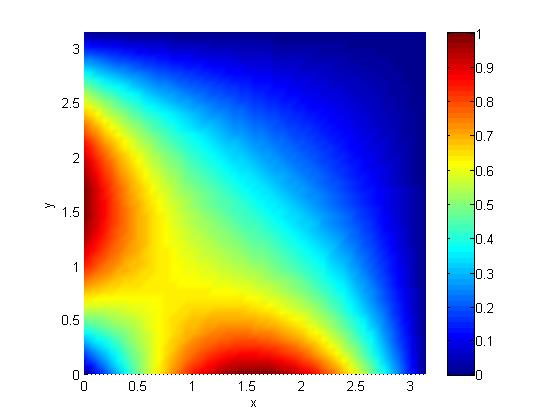
\includegraphics[width=7.3cm]{helm2.jpg}}
\subfigure[The 3-dimensional view of the temperature distribution]{
\label{1_2}
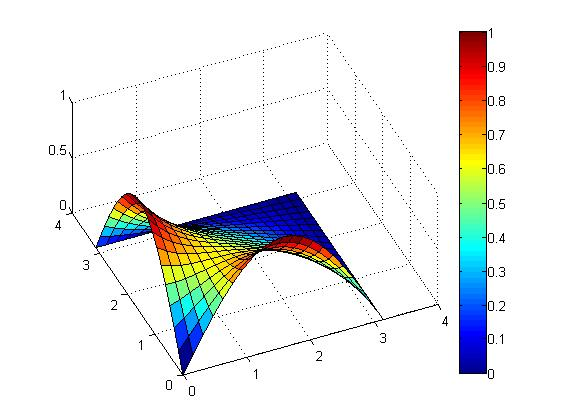
\includegraphics[width=7.3cm]{helm1.jpg}}
\caption{The numerical result of the Poisson Equation}
%\label{Fig.lable}
\end{figure}
\begin{table}[!htbp]
\centering
\caption{The Positive Correlation between tol and SSE}
\begin{tabular}{|l|l|l|l|l|l|l|}
\hline
 & ${M_x}$ & ${M_y}$ & $tol$ & $SSE$ & perror & err-order\\
\hline
 Case 1 & 50 & 50 & ${10^{ - 4}}$ & 0.1487 & 0.0172 & -1.8476\\
\hline
 Case 2 & 50 & 50 & ${10^{ - 5}}$ & 0.0033 & 0.0023 & -4.7496\\
\hline
 Case 3 & 50 & 50 & ${10^{ - 6}}$ & 0.0011 & 0.0014 & -5.5097\\
\hline
 Case 4 & 20 & 20 & ${10^{ - 4}}$ & $1.0859 \times {10^{ - 4}}$ & 0.0014 & -3.0674\\
\hline
 Case 5 & 20 & 20 & ${10^{ - 5}}$ & $9.3671 \times {10^{ - 5}}$ & $9.1363 \times {10^{ - 4}}$ & -0.5107\\
\hline
\end{tabular}
\end{table}
Thus, it is easy to observe the positive correlation between tol and SSE, also perror and err-order. Also, from the data, we may give an assumption that when ${M_x}$ and ${M_y}$ become larger, the increasing velocity of its accuracy level would become lower.
\subsection{Parabolic PDE}
As an example, we will deal with a special type of parabolic equation called one-dimensional heat equation, which is written as:
\begin{equation}
A\frac{{{\partial ^2}u(x,t)}}{{\partial {x^2}}} = \frac{{\partial u(x,t)}}{{\partial t}}\quad for\;0 \le x \le {x_f},\;0 \le t \le T
\end{equation}
with some boundary conditions(Dirichlet type) of $u(0,t) = {b_0}(t),\;u({x_f},t) = {b_{{x_f}}}(t)$, as well as the initial condition $u(x,0) = {i_0}(x)$.
And we will solve this equation using three methods which we mentioned above:\\
1. The Explicit Forward Euler Method\\
Here, we still use the iterative method:\\
first, define the function:
\begin{verbatim}
function [u,x,t] = heat_exp(a,xf,T,it0,bx0,bxf,M,N)
%solve a u_xx = u_t for 0 <= x <= xf, 0 <= t <= T
% Initial Condition: u(x,0) = it0(x)
% Boundary Condition: u(0,t) = bx0(t), u(xf,t) = bxf(t)
% M = # of subintervals along x axis
% N = # of subintervals along t axis
\end{verbatim}
second, we need to assign the value to $dx$ and $dt$:
\begin{verbatim}
dx = xf/M; x = [0:M]'*dx;
dt = T/N; t = [0:N]*dt;
\end{verbatim}
third, using the iterative method to do the numerical calculation:
\begin{verbatim}
for i = 1:M + 1, u(i,1) = it0(x(i)); end
for n = 1:N + 1, u([1 M + 1],n) = [bx0(t(n)); bxf(t(n))]; end
r = a*dt/dx/dx, r1 = 1 - 2*r;
for k = 1:N
for i = 2:M
u(i,k+1) = r*(u(i + 1,k) + u(i-1,k)) + r1*u(i,k); %Eq.(9.2.3)
end
end
\end{verbatim}
The \textsc{MatLab} routine \verb$heat_exp.m$ has been composed to implement this algorithm.\\
2. The Implicit Backward Euler Method\\
Similarly, first, define the function:
\begin{verbatim}
function [u,x,t] = heat_imp(a,xf,T,it0,bx0,bxf,M,N)
%solve a u_xx = u_t for 0 <= x <= xf, 0 <= t <= T
% Initial Condition: u(x,0) = it0(x)
% Boundary Condition: u(0,t) = bx0(t), u(xf,t) = bxf(t)
% M = # of subintervals along x axis
% N = # of subintervals along t axis
\end{verbatim}
second, we need to assign the value to $dx$ and $dt$:
\begin{verbatim}
dx = xf/M; x = [0:M]'*dx;
dt = T/N; t = [0:N]*dt;
\end{verbatim}
third, we need to do the matrix calculation, be careful that here we cannot use the iterative method we used before because the boundary condition is different.
\begin{verbatim}
for i = 1:M + 1, u(i,1) = it0(x(i)); end
for n = 1:N + 1, u([1 M + 1],n) = [bx0(t(n)); bxf(t(n))]; end
r = a*dt/dx/dx; r2 = 1 + 2*r;
for i = 1:M - 1
A(i,i) = r2;
if i > 1, A(i - 1,i) = -r; A(i,i - 1) = -r; end
end
for k = 2:N + 1
b = [r*u(1,k); zeros(M - 3,1); r*u(M + 1,k)] + u(2:M,k - 1); %Eq.(9.2.9)
u(2:M,k) = trid(A,b);
end
\end{verbatim}
  The \textsc{MatLab} routine \verb$heat_imp.m$ has been composed to implement this algorithm.\\
3. The Crank Nicholson Method\\
Similarly, first, define the function:
\begin{verbatim}
function [u,x,t] = heat_CN(a,xf,T,it0,bx0,bxf,M,N)
%solve a u_xx = u_t for 0 <= x <= xf, 0 <= t <= T
% Initial Condition: u(x,0) = it0(x)
% Boundary Condition: u(0,t) = bx0(t), u(xf,t) = bxf(t)
% M = # of subintervals along x axis
% N = # of subintervals along t axis
\end{verbatim}
second, we need to assign the value to $dx$ and $dt$:
\begin{verbatim}
dx = xf/M; x = [0:M]'*dx;
dt = T/N; t = [0:N]*dt;
\end{verbatim}
third, we need to do the matrix calculation, like the implicit Euler method, here we cannot use the iterative method.
\begin{verbatim}
for i = 1:M + 1, u(i,1) = it0(x(i)); end
for n = 1:N + 1, u([1 M + 1],n) = [bx0(t(n)); bxf(t(n))]; end
r = a*dt/dx/dx;
r1 = 2*(1 - r); r2 = 2*(1 + r);
for i = 1:M - 1
A(i,i) = r1;
if i > 1, A(i - 1,i) = -r; A(i,i - 1) = -r; end
end
for k = 2:N + 1
b = [r*u(1,k); zeros(M - 3,1); r*u(M + 1,k)] ...
+ r*(u(1:M - 1,k - 1) + u(3:M + 1,k - 1)) + r2*u(2:M,k - 1);
u(2:M,k) = trid(A,b); %Eq.(9.2.17)
end
\end{verbatim}
  The \textsc{MatLab} routine \verb$heat_CN.m$ has been composed to implement this algorithm.\\
And we will use an example to show you a comparison of these three methods.\\
\textbf{Example2} One-Dimensional Parabolic PDE: Heat Flow Equation.\\
Consider the Parabolic PDE:
\begin{equation}
\frac{{{\partial ^2}u(x,t)}}{{\partial {x^2}}} = \frac{{{\partial ^2}u(x,t)}}{{\partial {t^2}}}\quad for\;0 \le x \le 1,\;0 \le t \le 0.2
\end{equation}
with the initial condition and the boundary conditions:
\begin{equation}
u(x,0) = \sin \pi x,\;u(0,t) = 0,\;u(1,t) = 0
\end{equation}
The real solution of this equation is:
\begin{equation}
u(x,t) = {e^{ - {\pi ^2}t}}\sin (\pi x)
\end{equation}
Note that $\Delta x = 1/M$ and $\Delta t = 0.2/N$, thus the stability condition become:
\begin{equation}
\gamma  = \frac{{0.2{M^2}}}{N} \le \frac{1}{2}
\end{equation}
Choose $M = 3,6,12$ and corresponding $N = 6,24,96$, so in this case $\gamma = 0.3$, which satisfies the stability condition.
And the code of the example is:
\begin{verbatim}
%solve_heat
a = 1; %the parameter of (E9.2.1)
it0 = inline('sin(pi*x)','x'); %initial condition
bx0 = inline('0'); bxf = inline('0'); %boundary condition
xf = 1; M = 12; T = 0.2; N = 96; %r = 0.3
%analytical solution
uo = inline('sin(pi*x)*exp(-pi*pi*t)','x','t');
[u1,x,t] = heat_exp(a,xf,T,it0,bx0,bxf,M,N);
figure(1)
surf(t,x,u1);
colormap('jet');
view(3);
colorbar;
title('M=12 N=96 exp');
xlabel('t');ylabel('x');zlabel('T');
[u2,x,t] = heat_imp(a,xf,T,it0,bx0,bxf,M,N); %converge unconditionally
figure(2)
surf(t,x,u2);
colormap('jet');
view(3);
colorbar;
title('M=12 N=96 imp');
xlabel('t');ylabel('x');zlabel('T');
[u3,x,t] = heat_CN(a,xf,T,it0,bx0,bxf,M,N); %converge unconditionally
figure(3)
surf(t,x,u3);
colormap('jet');
view(3);
colorbar;
title('M=12 N=96 CN');
xlabel('t');ylabel('x');zlabel('T');
Uo = uo(x,t);
\end{verbatim}
Calculate the error:
\begin{verbatim}
error=0;
perror=0;
for i=1:(M+1)
    for j=1:(N+1)
        error=error+(Uo(i,j)-u1(i,j))^2;
        perror(i,j)=abs(Uo(i,j)-u1(i,j));
    end
end
error
k1=max(max(perror))
error=0;
perror=0;
for i=1:(M+1)
    for j=1:(N+1)
        error=error+(Uo(i,j)-u2(i,j))^2;
        perror(i,j)=abs(Uo(i,j)-u2(i,j));
    end
end
error
k1=max(max(perror))
error=0;
perror=0;
for i=1:(M+1)
    for j=1:(N+1)
        error=error+(Uo(i,j)-u3(i,j))^2;
        perror(i,j)=abs(Uo(i,j)-u3(i,j));
    end
end
error
k1=max(max(perror))
\end{verbatim}
And the result is:
\begin{figure}[H]
\centering
\subfigure[Explicit Euler]{
\label{inter1_1}
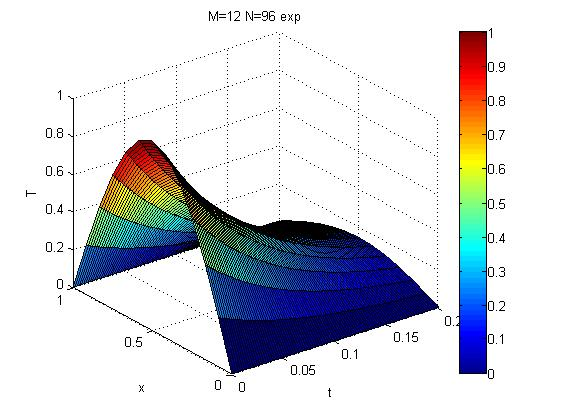
\includegraphics[width=7.3cm]{MNexp.jpg}}
\subfigure[Implicit Euler]{
\label{inter1_2}
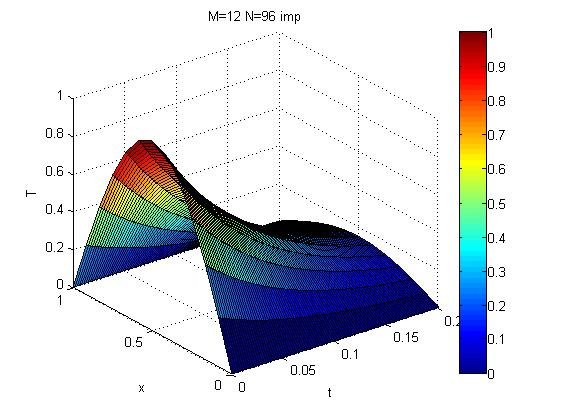
\includegraphics[width=7.3cm]{MNimp.jpg}}
\subfigure[Crank–Nicholson Method]{
\label{inter1_3}
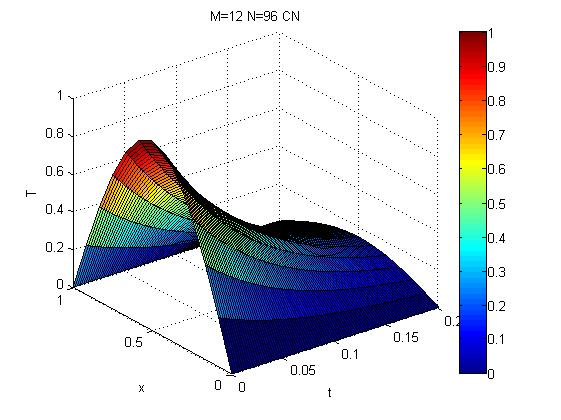
\includegraphics[width=7.3cm]{MNCN.jpg}}
\caption{Numerical result of the three methods}
%\label{Fig.lable}
\end{figure}
The comparison of different methods:
\begin{table}[!htbp]
\centering
\caption{The comparison of these three methods with M=12, N=96}
\begin{tabular}{|l|l|l|l|}
\hline
 & Explicit Euler & Implicit Euler & CN Method \\
\hline
 Point Error & 0.0017 & 0.0058 & 0.0021 \\
\hline
 SSE & 0.0012 & 0.0039 & 0.0018 \\
\hline
\end{tabular}
\end{table}
The comparison of different M and N:
\begin{table}[!htbp]
\centering
\caption{The comparison of different step length(CN Method)}
\begin{tabular}{|l|l|l|l|}
\hline
 & M=3, N=6 & M=6, N=24 & M=12, N=96 \\
\hline
 Point Error & 0.0269 & 0.0082 & 0.0021 \\
\hline
 SSE & 0.0066 & 0.0035 & 0.0018 \\
\hline
\end{tabular}
\end{table}
So, from the two tables, we may give out the assumption that:\\
1. CN method is a quite good method(at least better than implicit Euler method), and this is theoretically correct.\\
2. Smaller step length leads to higher accuracy level, which is quite reasonable because we can utilize more information of the PDE. \\
Also, if we let the $\gamma$ become very close to $0.5$ or even larger than it, we would see that the error would become very large for explicit euler method:
\begin{figure}[H]
\centering
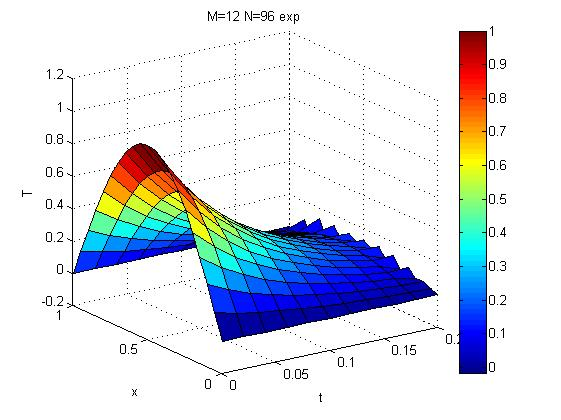
\includegraphics[width=9.6cm]{blow.jpg}
\caption{The result of the explicit euler}
\label{dis1_1}
\end{figure}
which obviously show the large error when $t$ become very close to 0.2.\\
This tells us that stability condition is very important to explicit euler method, however, the other two methods still working efficiently when it breaks up. Besides, if it converges, its accuracy may be better than that of the implicit backward Euler method, but generally no better than that of the Crank–Nicholson method.

\section{Contribution}
Luo Tao: Backgrounds
\\Wenchao Zhang: Definite Problem of Partial Differential Equation, numerical solution of iteration for PDE
\\Qikun Wu: Runge-Kutta method, matrix manipulation, solution to ODE system, typesetting with \AmS -\LaTeX
\\Jiale Wang: \textsc{MatLab} implementation of Elliptic and Parabolic PDE

\begin{thebibliography}{11}

  \bibitem[1]{Teschl}Gerald Teschl{\newblock} \tmtextit
  {Ordinary Differential Equations and Dynamical Systems}.{\newblock}  American Mathematical Society.{\newblock}

  \bibitem[2]{He&Peng}贺小明,彭名书{\newblock} \tmtextit
  {常微分方程与动力系统概论}{\newblock}
  北京理工大学出版社,2010.{\newblock}

  \bibitem[3]{Zhang&Xu}张贤科,许甫华{\newblock} \tmtextit
  {高等代数学}{\newblock}
  清华大学出版社,2008.{\newblock}
  
  \bibitem[4]{Lu&Guan}陆金甫,关治{\newblock} \tmtextit
  {偏微分方程数值解法}{\newblock}
  清华大学出版社,2004.{\newblock}
  
  \bibitem[5]{Peaceman&Rachford}Peaceman, D.W. and Rachford Jr, H.H.{\newblock} \tmtextit
  {The numerical solution of parabolic and elliptic differential equations}{\newblock}
  Journal of the Society for Industrial \& Applied Mathematics, vol 3, 28-41, 1955, SIAM.{\newblock}
  
  \bibitem[6]{Ambar}Ambar K. Mitra{\newblock} \tmtextit
  {Finite Difference Method for the Solution of Laplace Equation}{\newblock}
  Department of Aerospace Engineering, Iowa State University,2008.{\newblock}

\end{thebibliography}



\end{document}
